\documentclass{article}\usepackage{graphicx, color}
%% maxwidth is the original width if it is less than linewidth
%% otherwise use linewidth (to make sure the graphics do not exceed the margin)
\makeatletter
\def\maxwidth{ %
  \ifdim\Gin@nat@width>\linewidth
    \linewidth
  \else
    \Gin@nat@width
  \fi
}
\makeatother

\definecolor{fgcolor}{rgb}{0.2, 0.2, 0.2}
\newcommand{\hlnumber}[1]{\textcolor[rgb]{0,0,0}{#1}}%
\newcommand{\hlfunctioncall}[1]{\textcolor[rgb]{0.501960784313725,0,0.329411764705882}{\textbf{#1}}}%
\newcommand{\hlstring}[1]{\textcolor[rgb]{0.6,0.6,1}{#1}}%
\newcommand{\hlkeyword}[1]{\textcolor[rgb]{0,0,0}{\textbf{#1}}}%
\newcommand{\hlargument}[1]{\textcolor[rgb]{0.690196078431373,0.250980392156863,0.0196078431372549}{#1}}%
\newcommand{\hlcomment}[1]{\textcolor[rgb]{0.180392156862745,0.6,0.341176470588235}{#1}}%
\newcommand{\hlroxygencomment}[1]{\textcolor[rgb]{0.43921568627451,0.47843137254902,0.701960784313725}{#1}}%
\newcommand{\hlformalargs}[1]{\textcolor[rgb]{0.690196078431373,0.250980392156863,0.0196078431372549}{#1}}%
\newcommand{\hleqformalargs}[1]{\textcolor[rgb]{0.690196078431373,0.250980392156863,0.0196078431372549}{#1}}%
\newcommand{\hlassignement}[1]{\textcolor[rgb]{0,0,0}{\textbf{#1}}}%
\newcommand{\hlpackage}[1]{\textcolor[rgb]{0.588235294117647,0.709803921568627,0.145098039215686}{#1}}%
\newcommand{\hlslot}[1]{\textit{#1}}%
\newcommand{\hlsymbol}[1]{\textcolor[rgb]{0,0,0}{#1}}%
\newcommand{\hlprompt}[1]{\textcolor[rgb]{0.2,0.2,0.2}{#1}}%

\usepackage{framed}
\makeatletter
\newenvironment{kframe}{%
 \def\at@end@of@kframe{}%
 \ifinner\ifhmode%
  \def\at@end@of@kframe{\end{minipage}}%
  \begin{minipage}{\columnwidth}%
 \fi\fi%
 \def\FrameCommand##1{\hskip\@totalleftmargin \hskip-\fboxsep
 \colorbox{shadecolor}{##1}\hskip-\fboxsep
     % There is no \\@totalrightmargin, so:
     \hskip-\linewidth \hskip-\@totalleftmargin \hskip\columnwidth}%
 \MakeFramed {\advance\hsize-\width
   \@totalleftmargin\z@ \linewidth\hsize
   \@setminipage}}%
 {\par\unskip\endMakeFramed%
 \at@end@of@kframe}
\makeatother

\definecolor{shadecolor}{rgb}{.97, .97, .97}
\definecolor{messagecolor}{rgb}{0, 0, 0}
\definecolor{warningcolor}{rgb}{1, 0, 1}
\definecolor{errorcolor}{rgb}{1, 0, 0}
\newenvironment{knitrout}{}{} % an empty environment to be redefined in TeX

\usepackage{alltt}
\usepackage{times}
\usepackage{ie07}

\usepackage{graphicx}
\usepackage{subfig}

\usepackage{url}
\urlstyle{same}
%\usepackage[hidelinks]{hyperref}
\usepackage{hyperref}
\usepackage{amsmath}

%\setlength{\parskip}{6pt}

% put paranthesis after equation
% http://www.latex-community.org/forum/viewtopic.php?f=4&t=334
\makeatletter
\def\tagform@#1{\maketag@@@{\ignorespaces#1\unskip\@@italiccorr}}
\let\orgtheequation\theequation
\def\theequation{(\orgtheequation)}
\makeatother






\IfFileExists{upquote.sty}{\usepackage{upquote}}{}


\begin{document}

\title{AN OPEN SOURCE TOOL TO ESTIMATE MASS AND EFFICIENCY OF WIND TURBINE POWER TAKE-OFF SYSTEMS}

\authorname{Ozan Keysan, Markus A. Mueller}
\authoraddr{Institute for Energy Systems, University of Edinburgh, EH93JL, U.K.\\
Email: o.keysan@ed.ac.uk}

\maketitle

\keywords
Wind turbine, mass estimation, direct-drive, gearbox, generator, offshore

\abstract

This paper presents mass and efficiency estimations for wind turbine drive-train components. Data from literature and commercial catalogues are collected to obtain trend lines for each component. Different gearbox and generator types are investigated as well as the bearing and the low-speed shaft. An open-source tool is presented to compare different power take-off options in terms of weight and efficiency. The datasets and the user interface made available as an open source tool and can be accessed at GitHub.

\section{Introduction}

Far offshore wind turbines can help to exploit the wind energy resources that remained untapped so far. These turbines are planned to be installed as floating platforms due to  high water depths (\textgreater 40 m). Reliability and mechanical stability are the two most important issues for floating wind turbines. In particular, the nacelle mass is critical for the mechanical stability \cite{Christiansen2011, Sethuraman2013}. A higher tower head-mass increases the centre of mass significantly, and this should be balanced with a larger ballast, which increases the installation cost.

\vspace{6pt}

Although, doubly-fed induction generator coupled to a multi-stage gearbox is the most common power take-off (PTO) type for onshore wind turbines; it may not be the most suitable option for large offshore wind turbines. A direct-drive PTO system can be used to eliminate the gearbox, but the mass of a direct-drive generator can be larger than a high-speed PTO system depending on the power rating and the diameter.

\vspace{6pt}

In this study, data from manufacturers and literature are collected to predict the  mass and efficiency trend lines for wind turbine drive-train components. These equations are then used to build an open-source tool that can estimate the mass and efficiency of the total PTO system. Readers can access to datasets and modify the models using the tools defined in \autoref{access}.

\section{Power Take-Off Components}

The main components of the drive-train in a wind turbine can be listed as: bearing, shaft, gearbox, and generator. 

\subsection{Gearbox}

\subsubsection{Multi Stage Gearbox}

The most common gearbox type used in wind turbines is the three-stage gearbox, which increases the turbine speed to approximately 1500 rpm. 
Data from the following three-stage wind turbine gearbox manufacturers are collected: Bosch-Rexroth\cite{bosch}, Winergy\cite{winergy}, Moventas\cite{Moventas}, Eickhoff\cite{eickhoff}, and General Electric\cite{GE}, and plotted in \autoref{fig:gearbox}. From the figure, it may be seen that the mass of the gearbox is proportional to the input torque, which is represented as a linear function in \autoref{3G_gearbox}. 

\begin{knitrout}
\definecolor{shadecolor}{rgb}{0.969, 0.969, 0.969}\color{fgcolor}\begin{figure}[]


{\centering 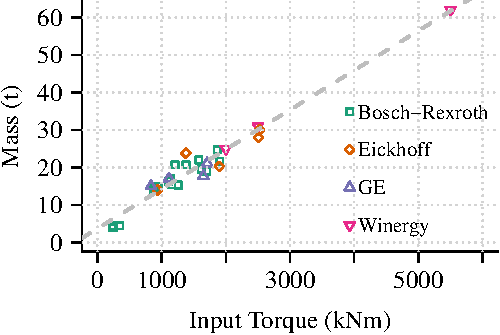
\includegraphics[width=\maxwidth]{figure/gearbox} 

}

\caption[Mass of three-stage gearbox versus input torque]{Mass of three-stage gearbox versus input torque.\label{fig:gearbox}}
\end{figure}


\end{knitrout}



\begin{equation}
\text{Mass(t)} = 0.011 \times T_{in(kNm)} + 3.7
\label{3G_gearbox}
\end{equation}

Multi-stage gearboxes usually consist of two planetary gear stages and an additional high-speed parallel-shaft helical gear stage. In \cite{Hau2005a} it is stated that each planetary gear stages have 1 \% power loss and each helical gear stages have 2 \% power loss. Thus, the efficiency of a three-stage gearbox can be approximated as in \autoref{3G_efficiency} \cite{Zhang2011a}. The equation implies that the efficiency of a three-stage gearbox varies from 97 \% at no load to 96 \% at full load.

\begin{equation}
  \text{Efficiency(\%)} = 97.0 - \dfrac{P_{in}}{P_{rated}}
  \label{3G_efficiency}
\end{equation}

\subsubsection{Single Stage Gearbox}

Gear ratios up to 15:1 can be achieved using a single stage gearbox \cite{Cotrell2002}. Single-stage gearboxes usually consist of a planetary stage with varying number of gears depending on the power rating. Single stage gearboxes have fewer gears and bearings than the multi-stage gearboxes, which increases the reliability. Moreover, their efficiencies are higher. In \cite{Matveev2011}, the efficiency of a single stage gearbox is given as:

\begin{equation}
  \text{Efficiency(\%)} = 99.5 - \dfrac{P_{in}}{P_{rated}}
\end{equation}

Mass of a single-stage gearbox coupled with medium-speed generator can be approximated as in \autoref{mass_1g}  \cite{Fingersh2006}. 

\begin{equation}
	\text{Mass(t)} = 0.088 \times {T_{in(kNm)}}^{0.774}
  \label{mass_1g}
\end{equation}


\subsection{Structural Components}

\subsubsection{Low Speed Shaft}
Low speed shaft connects the main hub to the gearbox or to the generator. Low speed shaft is not required for some drive train options (e.g. integrated bearing type). In \cite{Fingersh2006}, the mass and the cost of the low speed shaft is presented as a function of the turbine diameter. This equation can be modified as a function of the rated power as:

\begin{equation}
		\text{Mass (t)} = 1.35 \times {P_{rated(MW)}}^{1.44}
\end{equation}

\subsubsection{Main Bearing}

The mass of the main bearing can vary depending on the bearing type. For example, a double-tapered roller bearing for a direct-drive is heavier than a conventional two-point suspension type bearing. In  \cite{Fingersh2006}, the mass of the main bearing is presented as a function of turbine diameter. Assuming the mass of the bearing housing is equal to the bearing mass, the total mass of the main bearing system can be expressed as a function of the rated power as in \autoref{mass_bearing}.

\begin{equation}
	\text{Mass(t)} = 0.26 \times {P_{rated(MW)}}^{1.75}
  \label{mass_bearing}
\end{equation}

\subsection{Generator}

The generator types covered in this section are induction generators, permanent-magnet generators, synchronous generators, and superconducting generators. The cooling methods(air-cooled or water-cooled) for induction and synchronous generators are also included in the estimations. 

\subsubsection{Induction Generator}

Induction generator is the most common generator type used in wind turbines. Squirrel cage induction generators are preferred for small wind turbines, where doubly-fed induction generators are preferred for large wind turbines. Mass data for various 4-pole machines from ABB and Siemens catalogues are collected \cite{ABB2012a, Siemens}, which are plotted in \autoref{fig:induction_generator}. Trend lines for Siemens machines show that, the water-cooled induction generators are 18 \% lighter than the air-cooled machines. The mass of the induction generator as a function of the rated power can be expressed as in \autoref{mass-air} and \autoref{mass-water}.

\vspace{6pt}

Efficiencies of induction generators at rated load are plotted in \autoref{fig:induction_generator_efficiency}. The efficiency does not change with the cooling method, but increases with the power rating (efficiency increases from 96 \% to 97.5 \% as the power rating is increased from 2 MW to 8 MW). 

\begin{equation}
  \text{Mass}_{air-cooled}(t) = 3.91 \times {P_{rated(MW)}}^{0.69}
  \label{mass-air}
\end{equation}

\begin{equation}
  \text{Mass}_{water-cooled}(t) = 3.22 \times {P_{rated(MW)}}^{0.68}
  \label{mass-water}
\end{equation}

\begin{equation}
\text{Efficiency (\%)} = 95.64 \times {P_{rated(MW)}}^{0.01}
\end{equation}


\begin{knitrout}
\definecolor{shadecolor}{rgb}{0.969, 0.969, 0.969}\color{fgcolor}\begin{figure}[]


{\centering 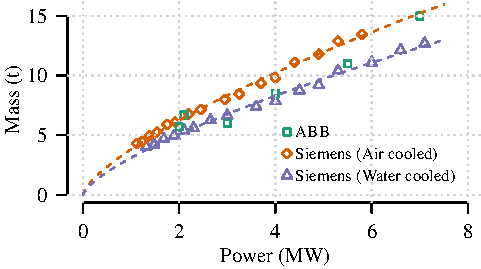
\includegraphics[width=\maxwidth]{figure/induction_generator} 

}

\caption[Mass of the induction generator vs torque]{Mass of the induction generator vs torque.\label{fig:induction_generator}}
\end{figure}


\end{knitrout}


\begin{knitrout}
\definecolor{shadecolor}{rgb}{0.969, 0.969, 0.969}\color{fgcolor}\begin{figure}[]


{\centering 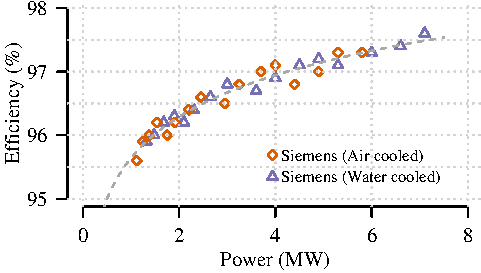
\includegraphics[width=\maxwidth]{figure/induction_generator_efficiency} 

}

\caption[Efficiency of induction generator at rated load vs power rating]{Efficiency of induction generator at rated load vs power rating.\label{fig:induction_generator_efficiency}}
\end{figure}


\end{knitrout}



\subsubsection{Direct-Drive Synchronous Generator}

Electrically excited direct-drive synchronous generators can be used in wind turbines to reduce the raw material cost compared to direct-drive permanent magnet generators. One example of such a machine is the 7.5 MW, 13 rpm Enercon 126 wind turbine, which has a generator mass of 220 t.
In \cite{upwind2011}, various direct-drive synchronous generator designs are presented from 0.75 MW to 10 MW. For direct-drive machines, it is better to calculate the mass as a function of the input torque, since the rotational speed varies with power rating. The linear equation that represents the mass of a direct-drive synchronous generator is given in \autoref{eesg_mass}.

\begin{equation}
  \text{Mass(t)} = 0.035 \times {T_{rated(kNm)}} + 8.9
  \label{eesg_mass}
\end{equation}

\subsubsection{Direct-Drive Permanent Magnet Generator}

Direct-drive permanent magnet generators have higher torque densities than electrically excited synchronous machines. Some notable direct-drive permanent magnet generators are: Harakosan (1.5 MW, 18 rpm, 47.2 t), The Switch (3.8 MW, 21 rpm, 81 t) \cite{Duan2009}. In \cite{Bang2008,upwind2011} many other permanent-magnet designs are presented. There are alternative designs to reduce the mass of PM machines, transverse-flux machine is being one of them, as presented in \cite{Bang2009}. However, radial flux permanent magnet machine is the most common topology, and therefore it is used for mass estimation in this section, which is given in \autoref{mass_ddpm}.

\begin{equation}
  \text{Mass(t)} = 0.028 \times {T_{rated(kNm)}} + 2.8
  \label{mass_ddpm}
\end{equation}

\subsubsection{Medium Speed Permanent Magnet Generator}

Permanent magnet generators can be coupled to single stage gearboxes to reduce the generator cost. They can can be fully-integrated to the gearbox to reduce the number of bearings, or can be semi-integrated for easy replacement. Data from ABB catalogues \cite{ABB2012} and Upwind project are collected and mass versus input torque graph is plotted in \autoref{fig:plot1gpm}. The equation of the trend line is shown in \autoref{mass_1gpm}. 

\begin{equation}
  \text{Mass(t)} = 0.031 \times {T_{rated(kNm)}} + 2.2
  \label{mass_1gpm}
\end{equation}

\begin{knitrout}
\definecolor{shadecolor}{rgb}{0.969, 0.969, 0.969}\color{fgcolor}\begin{figure}[]


{\centering 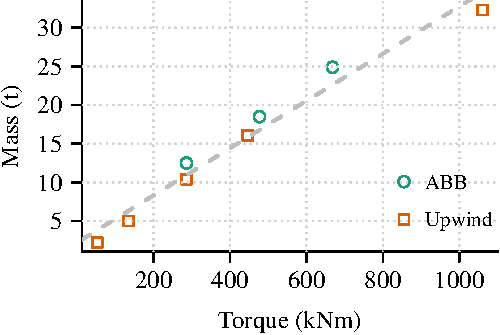
\includegraphics[width=\maxwidth]{figure/plot1gpm} 

}

\caption[Mass of the medium speed permanent magnet generator vs torque]{Mass of the medium speed permanent magnet generator vs torque.\label{fig:plot1gpm}}
\end{figure}


\end{knitrout}



% \begin{figure}[t]
%   \centering
%   \subfloat[Multibrid type 1 MW fully-integrated PM generator]{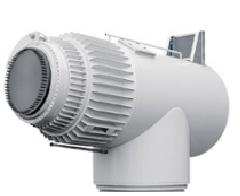
\includegraphics[width=0.2\textwidth]{images/abb_pm2}}
%   \subfloat[7 MW semi-integrated PM generator]{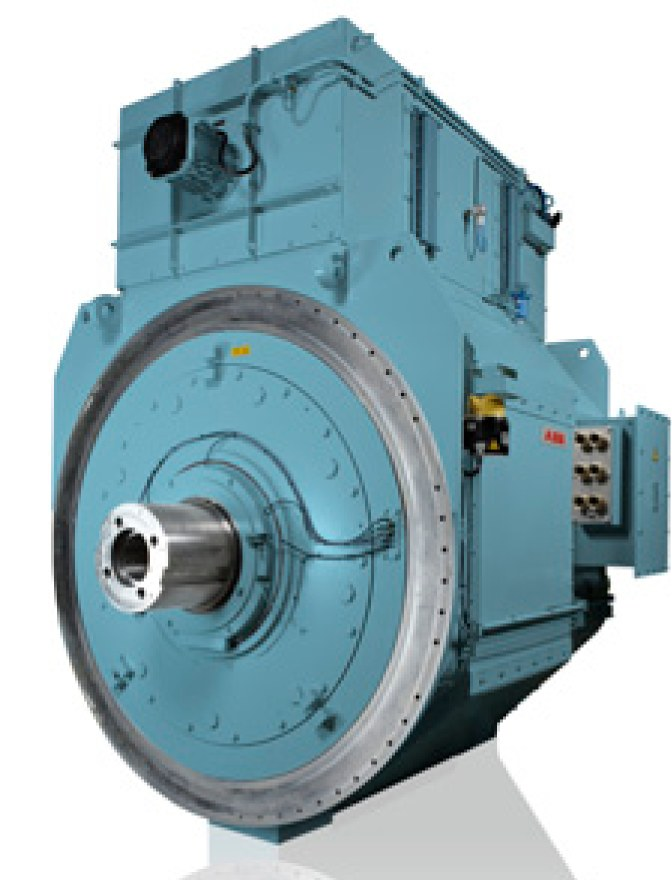
\includegraphics[width=0.18\textwidth]{images/abb_pm3}}
%   \caption{Medium speed permanent magnet generators. (Courtesy of ABB).} 
%   \label{abb_machines}
% \end{figure}

\subsection{Other Alternatives}

Hydraulic transmission is another option to increase the rotational speed of the turbine. Although, the efficiency of the hydraulic motors are low (especially at partial load), they can offer high torque densities. It is also possible to control hydraulic system in a way that, the electrical generator can be run at constant speed and can be directly connected to the grid. Data from H\"{o}ganas-Marathon catalogues are collected for high-torque applications \cite{Hagglunds2012} and the trend line is presented in \autoref{mass_hydraulic}. Note that, equation presents the mass of the hydraulic pump. The drive-train also requires a hydraulic motor, accumulators and an electrical generator.

\begin{equation}
  \text{Mass(t)} = 0.0042 \times {T_{rated(kNm)}} + 2.7
  \label{mass_hydraulic}
\end{equation}

Another novel concept is direct-drive superconducting generator, which can offer high-torque densities with a higher efficiency. Some commercial and conceptual direct-drive superconducting generators are compared in \cite{Keysan2011b}. The mass of a superconducting generator can be estimated using \autoref{mass_hts}.
%and it is stated that superconducting generators are lighter than direct-drive generators for torque requirements larger than 3000 kNm. 

\begin{equation}
  \text{Mass(t)} = 0.011 \times {T_{rated(kNm)}} + 45
  \label{mass_hts}
\end{equation}

\section{Open Source Tool}
\label{access}
All the equations presented in this study are combined in an open-source design tool, in which the user can select different PTO systems, and then define the input power and the rotational speed. The design tool estimates the mass and efficiency of the PTO system. The design tool, which the screen-shot is presented in \autoref{screenshot}, is currently built using Matlab GUI. It is planned to publish the design tool as a web application to remove software restrictions. 

\begin{figure}[t]
  \centering
  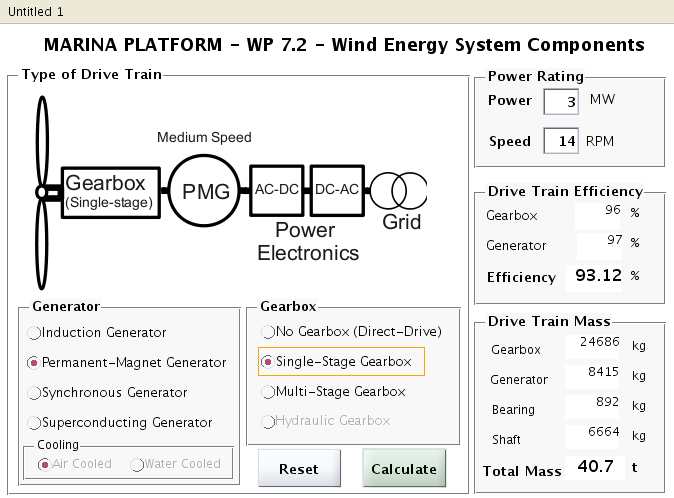
\includegraphics[width=0.5\textwidth]{images/marina_gui1}
  \caption{Screenshot of the user interface.} 
  \label{screenshot}
\end{figure}

\subsection{Accessing to Data and GUI}

All the datasets, graphs presented in this study are made available as open-source and can be accessed from the following GitHub repository: 

\begin{itemize}
  \item \url{http://github.com/ozank/wind-turbine-mass}
\end{itemize}

The readers are encouraged to add any available data to repository or modify the equations to improve the accuracy of the models.

\section{Conclusions}

In this study, the components of a wind turbine drive-train are investigated in terms of mass and efficiency. A user interface is developed to help designers to compare different PTO systems.  Currently, the design tool only covers the bearings, gearbox and generator. It is planned to include the turbine, hub, nacelle and power electronics in the future. All the work presented in this study is shared as an open-source tool and readers are encouraged to add extra information and modify the design tool.

\section*{Acknowledgements}
This work is supported by the FP7 project MARINA PLATFORM (Grant agreement number 241402). 

\bibliographystyle{plain}
\bibliography{IET_RPG_2013}
\noindent


\end{document}
